\chapter{Locomotion and Manipulation}\label{chap:locomotion}
Autonomous robots are systems that sense, compute, communicate, and actuate. Actuation, the focus of this chapter, is the ability of the robot to move and to manipulate the world. Specifically, we differentiate between locomotion\index{Locomotion} as the robot's ability to move and manipulation\index{Manipulation} as the robot's ability to move objects in the environment. Both activities are closely related: during locomotion the robot uses its motors to exert forces on its environment (ground, water or air) to move itself; during manipulation it uses motors to exert forces on objects to move them relative to the rest of the environment. This might not even require different motors. Insects are good examples for this: both can use their 6 legs not only for locomotion, but also for picking up and manipulating objects. The goals of this chapter are to:
\begin{itemize}
\item Introduce the concepts of locomotion, manipulation and their duality
\item Explain static vs.\ dynamic stability
\item Introduce ``degrees-of-freedom''
\item Introduce the forward kinematics of static manipulator arms
\end{itemize}

\section{Locomotion and Manipulation Examples}

Locomotion includes very different concepts of motion including rolling, walking, running, jumping, sliding (undulatory locomotion), crawling, climbing, swimming, and flying. They are drastically different in terms of energy consumption, kinematics, stability, and capabilities required by the robot that implements them. Yet, the above definitions are loose and ambiguous: for example, ``swimming'' can be done using many different forms of propulsion systems. Similarly, a sliding motion on the ground might result into swimming with only few modifications.

The way in which the individual parts of a robot can move with respect to each other and the environment is called the \emph{kinematics}\index{Kinematics} of the robot. Kinematics are only concerned with the position and speed (first derivative of position) of those parts, but not its \emph{dynamics}, which include acceleration (second derivative of position) and jerk (third derivative of position).

Commercially, the most dominant form of locomotion is rolling. This is due to the fact that rolling provides by far the most efficient energy-speed ratio (\cref{fig:todd}), making the invention of the wheel one of the greatest technological breakthroughs in history. Consequently, humans have modified their environment to have smooth surfaces of large extent such as the road network, but also warehouse and residential floors. In contrast, evolution has not evolved a single animal with wheel-like actuators.

\begin{figure}
	\centering
		\includegraphics[width=0.8\textwidth]{figs/todd85.png}
	\caption{Power consumption vs.\ speed for various means of locomotion. From \protect\citeasnoun{todd1985walking}.}
	\label{fig:todd}
\end{figure}


\begin{mdframed}Can you find examples of robots from the above categories? Identify the different types of actuators that are used in them.
\end{mdframed}

Most mechanisms capable of locomotion can also be used for manipulation with only minor modifications. Most industrial manipulators consist of a chain of rotary actuators that are connected by links. Most industrial robots have six or more independently rotating axes. We will see why further down below. Modern industrial manipulators have the ability to not only control the position of each of its joints, but precisely control the torque and force at each individual joint, making the arm arbitrary compliant, which is the inverse of stiffness in a mechanical sense. For dexterous manipulation a robot does not only need an arm, but also a gripper or hand. Grasping is a hard problem on its own and deserves its own chapter.

%This lecture focuses on the kinematics of simple mechanisms. Understanding the duality between locomotion and manipulation is important, however, to better introduce (and understand) concepts such as reference frames and forward kinematics.

\section{Static and Dynamic Stability}\label{sec:stability}
A fundamental difference between locomotion mechanisms is whether they are statically or dynamically stable\index{Static stability}\index{Dynamic Stability}. A statically stable mechanism will not fall even when all of its joints freeze (\cref{fig:stability}, left). A dynamically stable robot instead requires constant motion to prevent it from falling. Technically, stability requires the robot to keep its center of mass to fall within the polygon spanned by its ground-contact points. For example a quadruped robot's feet span a rectangle. Once such a robot lifts one of its feet, this rectangle becomes a triangle. If the projection of the center of mass of the robot along the direction of gravity is outside of this triangle, the robot will fall. A dynamically stable robot can overcome this problem by changing its configuration so rapidly that a fall is prevented. An example of a purely dynamically stable robot is an inverted pendulum on a cart  (\cref{fig:stability}, middle). Such a robot has no statically stable configurations and needs to keep moving all the time to keep the pendulum upright. While dynamic stability is desirable for high-speed, agile motions, robots should be designed so that they can easily switch into a statically stable configuration (\cref{fig:stability}, right).

\begin{figure}
	\centering
		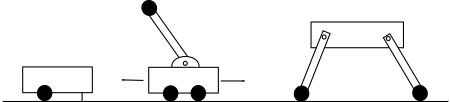
\includegraphics[width=\textwidth]{figs/stability.png}
	\caption{From left to right: statically stable robot. Dynamically stable inverted pendulum robot. Static and dynamically stable robot (depending on configuration).}
	\label{fig:stability}
\end{figure}

An example of a robot that has both statically and dynamically stable configurations is a quadruped (``four legs'') runner. Unlike walking, a running robot will always have two legs in the air and alternate between them faster than the robot could fall in either direction. Although statically stable walking is possible with only 4 legs, most animals (and robots) require 6 legs for statically stable walking and use dynamically stable gaits (such as galloping) when they have four legs. Six legs allow the animal to move three legs at a time while the three other legs maintain a stable pose.


\section{Degrees of Freedom}\label{sec:dof}
The concept of \emph{degree of freedom}\index{Degree of Freedom}, often abbreviated as DoF, is important for defining the possible positions and orientations a robot can reach. An object in the physical world can have up to six \bh{\emph{Cartesian}} degrees of freedom, namely forward/backward, sideways, and up/down as well as rotations around those axes. These rotations are known as pitch, yaw and roll and are illustrated in \cref{fig:pitchyawandroll}. \bh{These Cartesian degrees of freedom are distinct from the robot's mechanical degrees of freedom, which correspond to the number of points of actuation for a robot (i.e., a robotic arm with five joint motors is referred to as having five mechanical degrees of freedom).}

\begin{figure}
	\centering
		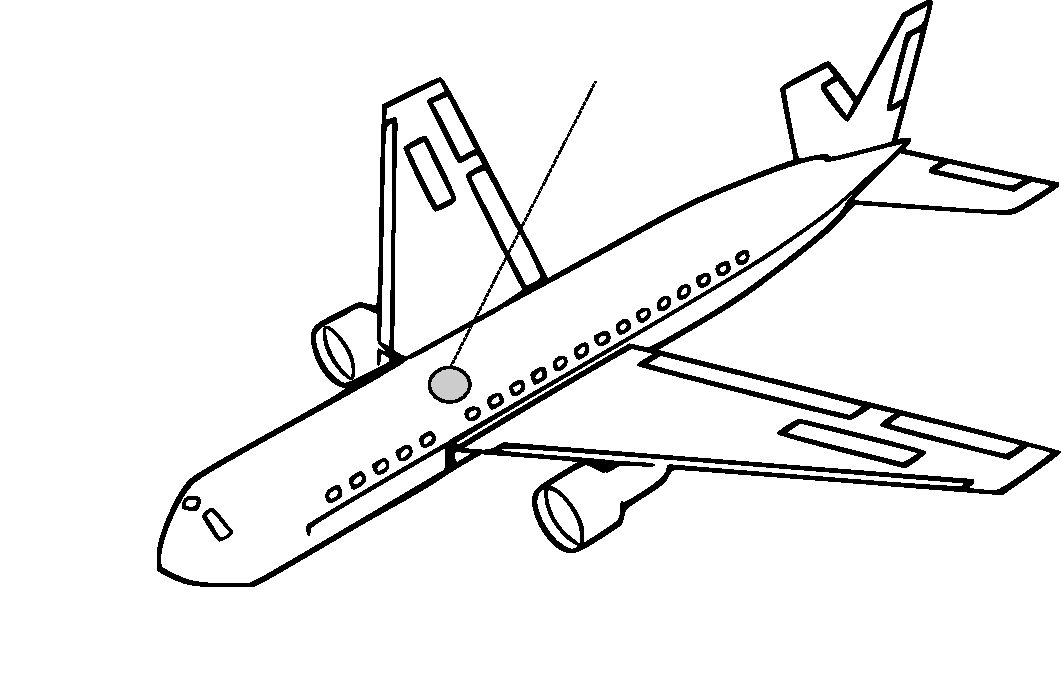
\includegraphics[width=\textwidth]{figs/pitchyawroll.png}
	\caption{Pitch, yaw and roll around the principal axis of an airplane.}
	\label{fig:pitchyawandroll}
\end{figure}

How many of those directions a robot can move in depends on the configuration of its actuators and the constraints the robot has with the environment. These relationships are not always intuitive and require more rigorous mathematical treatment (\cref{chap:kinematics}). The goal of this section is to introduce the degrees of freedom of standard mechanisms that are recurrent in robot design such as wheels or simple arms. For wheeled platforms, the degrees-of-freedom are defined by the types of wheels used and their orientation. Common wheel types are listed in \cref{tab:wheels}.

\begin{table}
\begin{tabular}{p{2.8cm}p{3cm}p{4cm}}
\hline
Wheel type & Example & Degrees-of-Freedom\\
\hline
Standard 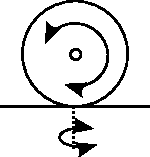
\includegraphics[width=2.5cm]{figs/wheeltype_standard.png} &	Front-wheel of a wheelbarrow	& Two
\begin{compactitem}
\item Rotation around the wheel axle
\item Rotation around its contact point with the ground
\end{compactitem}\\
\hline
Caster wheel	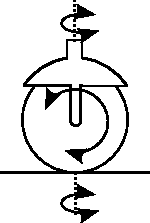
\includegraphics[width=2.5cm]{figs/wheeltype_caster.png}& Office chair & Three
\begin{compactitem}
\item Rotation around the wheel axle
\item Rotation around its contact point with the ground
\item Rotation around the caster axis
\end{compactitem}\\
\hline
Swedish wheel 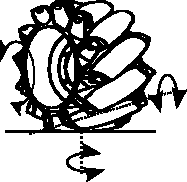
\includegraphics[width=2.5cm]{figs/wheeltype_swedish.png}& Standard wheel with non-actuated rollers around its circumference& Three
\begin{compactitem}
\item Rotation around the wheel axle
\item Rotation around its contact point with the ground
\item Rotation around the roller axles
\end{compactitem}\\
\hline
Spherical wheel 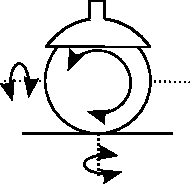
\includegraphics[width=2.5cm]{figs/wheeltype_spherical.png}& Ball Bearing & Three
\begin{compactitem}
\item Rotation in any direction
\item Rotation around its contact point
\end{compactitem}\\
\hline
\end{tabular}
\caption{Different types of wheels and their degrees of freedom. Adopted from \protect\citeasnoun{siegwart2011introduction},\label{tab:wheels}}
\end{table}

Only robots that use exclusively wheels with three degrees-of-freedom (3-DOF wheels) will be able to freely move on a plane. This is because the pose of a robot on a plane is fully given by its position (two values) and its orientation (one value). Robots that don't have wheels with three degrees of freedom will have \emph{kinematic constraints}\index{Kinematic constraints} that prevent them from reaching every possible point at every possible orientation. For example, a bicycle wheel can only roll into one direction and turn on the spot. Moving the bicycle wheel orthogonal to its direction of rolling is not possible, unless it is forcefully dragged (``skidding''), which requires more involved treatment not covered in this book. On the other hand, not having three degrees of freedom does not imply that some poses in the plane are unreachable, it may just require additional movements to achieve them.
A good analogue are figures on a chess-board. For example, a knight can reach every cell on a chess-board but might require multiple moves to do so. This is similar to a car, which can parallel park using back-and-forth motions. Instead, a bishop can only reach either black or white fields on the board, based upon its starting position.

Similar reasoning applies to aerial and underwater robots. Here, the position of the robot is affected by the position and orientation of thrusters, either in the form of jets or propellers, mounted on the robot. Things become complicated quickly, however, as the dynamics of the system are subject to fluid- and aerodynamic effects, which also change as a function of size of the robot. This book will not go into the details of flying and swimming robots, but the general principles of localization and planning will be applicable to them as well.

\begin{mdframed}Think about possible wheel, propeller and thruster configurations. Don't limit yourself to robots, but consider also street and aerial vehicles and be creative --- if you can think about a setup that makes sense, i.e., allows for reasonable mobility --- somebody will already have built it and analyzed it. What are the advantages and disadvantages of each?
\end{mdframed}

For manipulating arms, Cartesian degrees of freedom refer to the positions and orientations (rotations around the primary axes) that the end-effector can reach. Each actuated joint will typically add a degree of freedom, unless it is redundant (moving in the same direction, with the same physical effect, as a different joint). \cref{fig:basickinematics} shows a series of manipulators operating in a plane. By this, the degrees of freedom of the end-effector are limited to moving up and down, sideways, and rotating around its pivot point. As a plane only has those three degrees of freedom, adding additional joints cannot increase the Cartesian degrees of freedom unless they allow the robot to also move in and out of the plane.

An exact definition of the number of degrees of freedom is tricky and requires deriving analytical expressions for the end-effector position and orientation, which will be subject to \cref{chap:kinematics}.

\begin{figure}
	\centering
		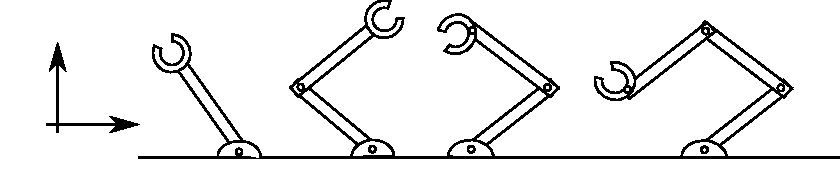
\includegraphics[width=\textwidth]{figs/basickinematics.png}
	\caption{From left to right: Manipulators with one, two, three and three DOF. The degrees of freedom of moving in a plane are the position of the end-effector with respect to its height and displacement with respect to the base, as well as its orientation.}
	\label{fig:basickinematics}
\end{figure}

Choosing the ``right'' kinematics is a trade-off between mechanical complexity, maneuverability, achievable precision, cost, and ease of control. The very popular differential-wheel drive consisting of two independently controlled wheels that share a common axis such as on the iRobot Roomba is cheap, highly maneuverable and easy to control, but makes it hard to drive in a straight line. This requires both motors to turn at the exact same speed and both wheels to have the exact same diameter, which is hard to achieve in practice. This problem is solved well by car-like steering mechanisms, but they have poor maneuverability and are difficult to control (think parallel-parking).


\section*{Take-home lessons}

\begin{itemize}
\item In order to perform planning for a robot, it's necessary to understand how its control parameters map to actions in the physical world.
\item The kinematics of a robot are fully defined by the position and orientation of its wheels, joints and links no matter whether it swims, flies, crawls or drives.
\item Many robotic systems cannot be fully understood by considering kinematics alone, but require you to model their dynamics as well. This book will be limited to modeling kinematics, which is sufficient for low-speed, mobile robots and arms.
\end{itemize}


\section*{Exercises}\small
\begin{enumerate}
\item What are the Cartesian degrees of freedom of a push lawnmower with four wheels? How is it still possible to mow an entire lawn with one, even though the wheels don't yaw?
\item Is a car statically or dynamically stable? What about a motorcycle?
\item What are the Cartesian degrees of freedom of an office chair with all caster-wheels?
\item What are the maximum Cartesian degrees of freedom for orientable objects driving on the plane?
\item What are the maximum Cartesian degrees of freedom for objects that can freely translate and rotate in the world?
\item Calculate the Cartesian degrees of freedom of a differential drive robot with two powered rear wheels and a central, front-mounted caster wheel. What happens when you add a second caster wheel?
\item Calculate the Cartesian degrees of freedom of a standard car. How is it possible to still reach every point on the plane?
\item A steering wheel allows you to change the yaw of your car. Can you also change its pitch and its roll?
\end{enumerate}\normalsize
